\documentclass{report}
\usepackage{fancyhdr}
\usepackage{graphicx}
\usepackage{url}
\usepackage[semicolon]{natbib}
\usepackage{amsmath}
\usepackage{adjustbox}
\usepackage{babel,blindtext}


\usepackage{tikz,pgfplots,pgf}
\usetikzlibrary{matrix,shapes,arrows,positioning}

\fancyhead{}
\fancyhead[LO, LE]{\rightmark}

\title{
	\begin{center}
	\includegraphics[width=3cm]{Images/covlogo.png} \\
	\vspace{2mm}
	{Convolutional Neural Network-based medical checkup system for Pigmented Skin Lesions Classification.} \\
	\vspace{5mm} %5mm vertical space
	\large {
		{School of Computing, Engineering and Mathematics}\\
		{Coventry University}\\
	}
	\vspace{3mm} %3mm vertical space
	\textbf{ Bsc Computer Science}\\
	{\large Project Supervisor: Dr.David Croft}\\
	{\large Submission Date: 21/04/2020} \\
	\end{center}
}
\author{
	{\large Author Name:  Vinayak Sareen} \\
	{\large Student Id Number:  7651331} \\
	{\large Ethics Application Number: P101878 }\\
}
\date{}
\pagestyle{fancy}
\begin{document}
\maketitle

\chapter*{Statement of originality}
\subsection*{Declaration of originality}
I Declare that This project is all my own work and has not been copied in part or in whole from any other source except where duly acknowledged.  As such, all use of previously published work (from books, journals, magazines, internet etc.) has been acknowledged by citation within the main report to an item in the References or Bibliography lists. I also agree that an electronic copy of this project may be stored and used for the purposes of plagiarism prevention and detection.
\subsection*{Statement of copyright}
I acknowledge that the copyright of this project report, and any product developed as part of the project, belong to Coventry University. 
Support, including funding, is available to commercialise products and services developed by staff and students. 
 Any revenue that is generated is split with the inventor/s of the product or service. 
For further information please see www.coventry.ac.uk/ipr or contact ipr@coventry.ac.uk.
\subsection*{Statement of ethical engagement}

I declare that a proposal for this project has been submitted to the Coventry University ethics monitoring website (https://ethics.coventry.ac.uk/) and that the application number is listed below \\
\\ 
\underline{Sign}: \textbf{Vinayak Sareen}. \hspace{20mm} \underline{Date}:  \textbf{07/03/20}
\pagebreak
\subsection*{}
\begin{center}
    \textbf{Project Details }\\
    \vspace{2mm}
\begin{tabular} {| c | c |}
	\hline
    FirstName: &Vinayak \\
    LastName: & Sareen \\
    Student ID Number & 7651331 \\
    Ethics Application Number & P101878 \\
    Supervisor Name & Dr.David Croft \\
    \hline
\end{tabular}
\end{center}


\chapter*{Abstract}
Abstract should be a succinct and self-standing summary of the basis, context and achievements of the project. Minimally an abstract does three things: (1) It states the problem that you set out to solve, (2) It describes your solution and method, (3) It states a conclusion about the success of the solution. Be straightforward and factual and avoid vague statements, confusing details and "hype". Do not be tempted to use acronyms or jargon to keep within the half-page limit. Consider that search engines, librarians and non-computer scientists wishing to classify your Report rely on the abstract. You may if you wish provide a short list of keywords (2-6 is reasonable) at the end of the abstract.

\tableofcontents

\chapter*{Acknowledgements}
I want to express my gratitude to my supervisor Dr David Croft for guiding me thought the investigations. The support of all medical professionals who contribute by providing data to the research is sincerely acknowledged. At last, I would thank my parents, who supported me finically and psychologically throught this journey of computer science.

\chapter{Introduction}
\section{Introduction to Problem}
\paragraph*{}

Skin cancer is categorized into two types: melanoma and non-melanoma skin cancer. 
Melanoma, is the most dangerous kind of skin cancer accounted for an estimated 16,000 deaths 
each year from 2014 to 2016 in the United Kingdom (Cancer Research UK, 2020). 
The melanoma tumour caused by melanocytes can result in uncontrolled and abnormal growth which 
can spread in the human body \citep*{KOROTKOV201269}.
Detection and classification of unknown pigmented skin lesions can result in early diagnosis 
of the medical problem. The research data provided by cancer research organisation in 2017 has 
shown that melanoma was the 20th most common disorder with new incidents of 81,00 and 83,00 in males 
and females respectively in the United Kingdom \citep*{KOROTKOV201269}. 
Dermoscopy is a non-invasive method of examining the pigmented skin, which includes microscopic imaging of the surface structure of pigmented
skin lesions \citep*{KOROTKOV201269}.
Early diagnosis of pigmented skin lesions is crucial to classify skin disorders to decrease mortality concerning particular skin disorders. Dermoscopy improves the detection of melanoma compared to detection of disease with naked eyes by analysing the pigmented skin lesion. Previous studies have shown that such tumours can result in higher chances of better treatment and cure of disease by removing the tumour \citep*{CELEBI2007362}.
The current diagnosis method of detection involves using ABCD rule which considers the Asymmetry, Border irregularity, Colour irregularities, Darmascopic structures respectively of common pigmented skin lesions \citep*{LOESCHER2013170}.
People working in busy work environments or less mobility can be victims of belated and slow diagnosis of such dangerous skin cancers.
The automated analysis of pigmented skin lesions using artificial neural networks can be beneficial in optical analysis of microscopic images of pigmented skin lesions. 
The primary targeted audience who benefits from the outcome is the people who are working in busy work environments or people with less mobility are best to use cases which can use such an automated system. Booking a prior appointment with medical professionals based on the urgency of detected medical problems can result in the immediate treatment of patients with more critical conditions. The people with less mobility such as older audiences or people with special needs can detect pigmented skin lesions through online systems in an inconvenient manner. Medical institutions can use such technologies to automate the process of pre-health checkups and overcome the problem of shortage of staff members in case of emergency. Such automated systems can also result in faster diagnosis of medical problems compared to a manual analysis by a clinician. 
Furthermore, manufacturing companies which supply the microscopic medical instruments can also use such intelligent models with their products to provide value to customers and medical institutions.

\section{Objective of Research}
The research concentrates on developing a type of artificial neural network called a convolutional network to perform automated optimal analysis to identify the class of pigmented skin lesion. 
The research focuses on providing the quantitative analysis on comparing the results predicted by the automated intelligent machine are compared with medical professionals to identify the classes of pigmented skin lesions. The study employs different experiments by applying different model architectures and analysing accurate hyper-parameters for optimal performance. 
The research concentrate on analysing limited skin tumours such as melanoma, 
benign keratosis, melanocytic nevi and basal cell carcinoma. 
The investigation employs publicly available HAM10,000 dataset \citep*{DVN/DBW86T_2018}. 
The extensive collection of 10,000 images of labelled data units were collected from a diverse population of subjects over twenty years.
The outcome of the research project will to be analyse the effectiveness of the automated pigmented 
lesion system. Furthermore, the intelligent model will be deployed on web based system to provide 
interface to use the system to analyse by general audience.
\pagebreak
\pagebreak

\section{Perceptron Model}
\subsection{Inspiration from biological Structure of Neurons}
The human brain are componsed of millions specialised cell "neurons" which are interconnected to each other which carry electrical and chemical signals from neuron to another to function
There are an estimated 500 trillion connections between neurons in the human nervous system which helps communicate signals \citep*{patterson2017deep}.
The inspiration of artifical neural networks are taken from functioning of human brain and learn to recoganise patterns and relationship in the data \citep*{AGATONOVICKUSTRIN2000717}. 
\subsection{Neural Structure}
\vspace{3mm}
\begin{center}
  \includegraphics[width=10cm]{Images/neuron.png}
\end{center}

The image above represents the biological structure of the neuron which includes three major parts of a neuron dendrite, nucleus and axon terminals.
The dendrites are accountable for accepting the incoming signals from other neurons. 
Moreover, nucleus of the neuron is responsible for processing the information. 
Furthermore, the processed information gets passed to other neuron or organs through axon terminals 
in the human body \citep{AGATONOVICKUSTRIN2000717}. 
 
\subsection{Perceptron Model}

\begin{center}
    \includegraphics[width=0.6\textwidth]{Images/p_model.png} \\
\end{center}
\vspace{2mm}
Preceptron model was proposed by Frank Rosenblatt in 1943 to design the model to 
mimic the human brain \citep{939589}. Preceptron model or single layered feed forwards network 
networks takes the vectors of inputs and multiply with a randomly 
initialised weights and add random bias to network and process the information by providing data to the
activation function to process the information \citep{AGATONOVICKUSTRIN2000717}.
Figure above represents the simple preceptron model which consists inputs x and weights w 
for which weighted sum of muliplication result of 
inputs and weights will be passed to step activation function.

\subsection{Mathematical Representation }
\vspace{3mm}
{The equation below represents the preceptron model mentioned above in Mathematical notations.}
\begin{equation}
    \begin{split}
        y = \Big[\sigma(\sum_{k=0}^n x_k.w_k + b_k)\Big] \\
    \end{split}
\end{equation}

     {
        In, euation above ${\sigma = Activation function}$, x and w represents the inputs provided 
        and weights vectors in the network respectively. Furthermore symbol b represents the  bias in the equation, 
        during the optimisation of the network weights and bias are adjusted accordingly to improve the 
        predection. There are various activation functions ${\sigma}$ such as  step function sigmoid, 
        relu, leaky relu and others that can be applied based on the requirments of model prediction.
    }
\pagebreak
\section{Multi Layered Feed Forward Neural Network}
\begin{center}
    \begin{figure}[htp]
        \centering
        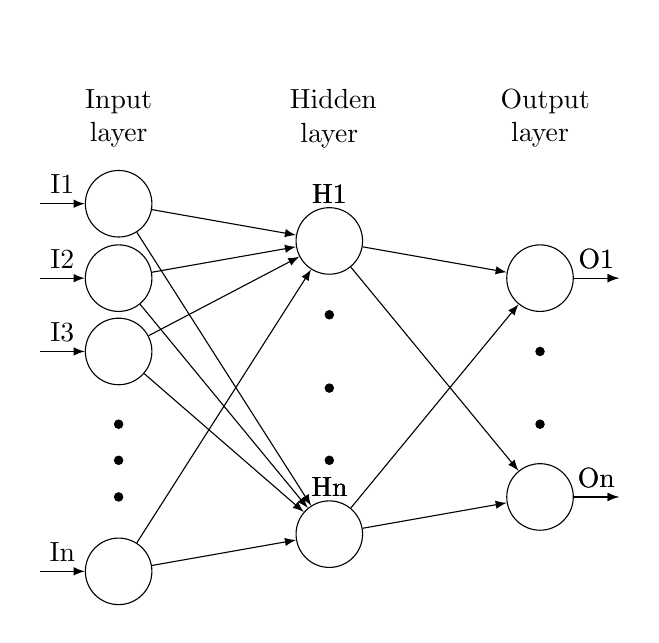
\begin{tikzpicture}[
        plain/.style={
          draw=none,
          fill=none,
          },
        dot/.style={draw,shape=circle,minimum size=3pt,inner sep=0,fill=black
          },
        net/.style={
          matrix of nodes,
          nodes={
            draw,
            circle,
            inner sep=8.5pt
            },
          nodes in empty cells,
          column sep=0.6cm,
          row sep=-11pt
          },
        >=latex
        ]
        \matrix[net] (mat)
        {
        |[plain]| \parbox{1cm}{\centering Input\\layer} 
                  & |[plain]| \parbox{1cm}{\centering Hidden\\layer} 
                               & |[plain]| \parbox{1cm}{\centering Output\\layer} \\
                  & |[plain]|                 \\
        |[plain]| &            & |[plain]|    \\
                  & |[plain]|  &              \\
        |[plain]| & |[dot]|                   \\
                  & |[plain]|  & |[dot]|      \\
        |[plain]| & |[dot]|    & |[plain]|    \\
        |[dot]|   & |[plain]|  & |[dot]|      \\
        |[dot]|   & |[dot]|    & |[plain]|    \\
        |[dot]|   & |[plain]|  &              \\
        |[plain]| &            & |[plain]|    \\
                  & |[plain]|                 \\
        };
        \foreach \ai/\mi in {2/I1,4/I2,6/I3,12/In}
          \draw[<-] (mat-\ai-1) -- node[above] {\mi} +(-1cm,0);
        \foreach \ai in {2,4,6,12}
        {\foreach \aii/\mii in {3/H1,11/Hn}
          \draw[->] (mat-\ai-1) -- (mat-\aii-2) node[yshift=0.6cm] {\mii};
        }
        \foreach \ai in {3,11}
        {  \draw[->] (mat-\ai-2) -- (mat-4-3);
          \draw[->] (mat-4-3) -- node[above] {O1} +(1cm,0);}
        \foreach \ai in {3,11}
        {  \draw[->] (mat-\ai-2) -- (mat-10-3);
          \draw[->] (mat-10-3) -- node[above] {On} +(1cm,0);}
        \end{tikzpicture}
        
        \caption{Multi Layered Neural Network diagram.}
        \label{fig_m_3}
        \end{figure}
\end{center}

The perceptron model acts as the base for all the functioning of modern multi-layered neural networks.
The output of the single neuron described in the above perceptron is taken as the input in the next layer of the network. The above figure(1.1) shows an example of multi-layered neural where the first layer is known 
as input layer and intermediate layers are called hidden layers and the last layer is known as the output layer.
The single neuron can perform limited computation but the computation power increases with inter-connected
neurons in the network \citep{AGATONOVICKUSTRIN2000717} where at each layer information is processed through the appropriate 
activation function. Artificial neural networks are designed to learn the patterns and relationships in the data and requires enough amount of data to train and predict accurate outputs \citep{AGATONOVICKUSTRIN2000717}.
The training data is passed to the neural network to recognise the patterns in data and each iteration or epoch 
the model prediction gets improved with the optimisation algorithm which propagates through the network to 
update the weights and bias to increase the accuracy \citep{AGATONOVICKUSTRIN2000717}. The accuracy of the neural networks are determined through various hyper-parameters such as learning rate, number of hidden layers in the model and 
number of epochs for which the model is trained. The fundamental rule for learning in artifical model 



\pagebreak
\subsection{Cost Function and Backpropagation Algorithm}
The objective for training deep learning models is to reduce
the error in prediction on each iteration and 
learn data patterns and relationships by increasing the 
prediction accuracy. Cost function is an appropriate method to 
analyse the performance of the neural network as it describes 
how well, model is predicting the actual results. The equation below 
describes the cost function equation also known as mean squared error \citep{7013173}.
\vspace{2mm}

\begin{center}
\begin{equation}
    c = \frac{1}{2m} \sum_{i=1}^m(h - y)^2
\end{equation}
\end{center}

In, equation(1.2)  h is the predected outcome of the intelligent model 
and y is the actual value of the input. The equation above is mean square of 
predected value - actual value. The objective of optimisation algorithms is 
minimise the equation(1.2) to decrease the value of cost function so, the value is 
close to zero as much as possible so, that predected and actual 
value are almost same which means overall model accuracy has improved \citep{7013173}.

\begin{figure}[!htp]
    \centering
    \includegraphics[width=\textwidth]{Images/gd.png}
    \caption{Gradient Descent}
\end{figure}

Gradient descent algorithm  is a optimisation algorithm which is iterative in nature aims 
to minimise the cost function is gradient descent. The algorithm functions by minimising the objective 
function in the space. 

\begin{center}
    \begin{equation}
            \frac{\partial }{\partial w} (\frac{1}{2m} \sum_{i=1}^m(h - y)^2)
    \end{equation}

    \begin{equation}
        \frac{\partial }{\partial b} (\frac{1}{2m} \sum_{i=1}^m(h - y)^2) 
    \end{equation}
\end{center}


The algorithm functions by finding the 
partial deravative of the cost function in respect to weights and bias as shown in the equations (1.3) and  (1.4) above.
The objective is to find minmum of the cost fuction which improves the accuracy \citep{7013173}. 
Backpropagation utilises the gradient descent algorithm and propgates after each layer to 
update the bias and weights in backwards direction to improve accuracy of the model.


\chapter{Literature Review}
\subsection{Convential Diagnosis Methods}

The most common conventional diagnosis method of detection involves
using ABCD rule which considers the Asymmetry, Border irregularity, Colour
irregularities,  Darmascopic structures respectively of common pigmented skin
Lesions \citep*{LOESCHER2013170}. The above method of analysis is performed on dermoscopic images of pigmented 
skin lesions.  Dermatoscopy is non-invasive microscopic imaging of
 pigmented skin lesions which provides clear imaging to perform 
 proper analysis on pigmented skin lesions \citep*{LOESCHER2013170}. 
 Furthermore, the result of dermatoscopic images is examined 
 by dermatologists to classify the pigmented skin lesion.  

\subsection{Support Vector Based Machine}
Thompson Felsia and Jeyakumar proposed research in 2017 on 
support vector machine based classifier to detect multi-lesions skin cancer by analysing pigmented skin lesions with an accuracy of 86.37 percent.
The proposed investigation with SVM based classifier has performed image segmentation using SRM (support region merging) algorithm. Furthermore, it employs SURF (speed up robust features) to find the region 
of interest for feature extraction to get optimal classification performance based on vector-based technique \citep*{thompson2017vector}. 
However, the research does not include image augmentation which generalises the predictions accurate to test in 
real-world environment. The research papers mention that support vector machine for automated classification of pigmented skin lesions is sensitive to the artefacts and can 
potentially increase the false positives which mean that predicted result for analysis was wrong positive prediction instead of an actual negative result. The investigation will perform image augmentation to generate random 
samples of images with different rotation angle and flipped images will be used to train and test the model to generalise the overall performance.

\subsection{Border Detection Based System}
Rahil Garnavi and his other co-researchers purposed research based on a state of the art border detection method combined with the colour space analysis and clustering-based histogram hybrid thresholding to classify pigmented skin lesions.
 The research was primarily focused on the research was to develop the hair removal mechanism to perform colour channels transformation. Furthermore, for all the image channels the noise reduction 
and clustering-based histogram thresholding were performed for optimal border detection. The predicted outcomes of novel broder detection system were compared with the 
borders detected by the actual dermatologists on a sample of 
dermoscopic pigmented skin lesions to understand the reliability of the 
system \citep*{GARNAVI2011105}.However, the system was only tested on a data sample set of 
30 dermoscopic images and four sample sets of dermatologist hand-drawn images were used as ground truth to compare the results. The system was tested on overall 85 dermoscopic images.
Border detection can be used to analyse the pigmented skin lesions but convolutional networks have the potential to find more data patterns in the images to minimise the cost function 
using the backpropagation algorithm. The current research will 
employe basic image segmentation based on the binary threshold 
algorithm as an experiment to help network detecting more accurate
borders of pigmented skin lesions.

\subsection*{Deep Feature to classify Pigmented Skin lesions}

In 2016, a research paper from Simon Fraser University’s computer science and medical image analysis lab had researched using 
deep residual network architecture with ten labelled 
classes of pigmented skin lesions. The research was based on very 
deep convolutional network architecture with the accuracy 
of 85.8 percent in classifying five distinct classes and
81 percent in classifying 10 classes of pigmented skin lesions
\citep*{7493528}. Although the performance of the overall convolutional network was accurate, the training and testing data were limited to 13,00 overall images of 10 distinct classes.
 However, In the current research project, the classes of labelled images will be five and around 9,000 overall images will be used during the investigation.
 Estimated 80 percent of data will be consumed for training the model, and the rest of the label images will be used as validation and testing datasets 
 to evaluate the performance of the model. 
 Research is also consuming such artificial neural network-based technologies to various areas of investigations.

\chapter{Methodology}
The research purposes a solution based on deep convolutional neural networks with various experiments mentioned in further sections. The operations require machine learning specific configuration for Cuda libraries and configuration to run programs on available GPU(Graphical Processing Unit) for faster processing and further, instructions to setup environment can be found at \url{https://www.tensorflow.org/install/gpu}. In addition, jupyter notebooks were used in these experiments, which provides an appropriate interface to experiment and write markdowns. The data science and machine learning libraries such as NumPy for numerical operations, matplotlib for visualisation, Keras for developing deep learning models and OpenCV for image processing was used in the process of developing an automated system for classifying pigmented skin lesions. HAM,1000 dataset was used to train image classifier, which can be found at
\url{https://dataverse.harvard.edu/dataset.xhtml?persistentId=doi:10.7910/DVN/DBW86T}. The dataset contains two folders containing dermatoscopic images of pigmented skin lesion and CSV file which contains meta information and image name for each pigmented skin lesion.

\section*{Data Prepration}
The information present in the dataset for not in a usable form. Datasets contain unclear and hairy images of pigmented skin lesions which were manually removed from the dataset to enhance the quality of available data. The information was read using pandas into the data frame, which is a data structure that allows storing tabular data from CSV files. The CSV file contained irrelevant information such as gender and age of patients and unbalanced data classes data columns were dropped from the dataset. Furthermore, the dataset was divided into training and testing sets using \url{sklearn.model_selection.train_test_split} class in the portion of 80 per cent for the training dataset and 20 per cent of testing datasets. The next step towards to preparing the dataset was reading the images data into NumPy array for both training and testing datasets and converting the image names from pandas series to NumPy array corresponding to each image in the dataset.

\chapter{Evaluations and Results}
In this chapter, you should evaluate what you have done, and say what answer (to your research question) you have arrived at. It may be that in your method you describe some experiments, and this section records your results and analysis of those results. This is an important section -- most students gain or lose marks in either their literature review or evaluation. The key to producing a convincing evaluation is to plan very early in the project what information or results you will need to write this section.

\chapter{Project Managment}
\subsection*{Meeting Logs with Supervisor}
\subsection*{Software Development Lifecycle}
\subsection*{Work Managment System}
\begin{figure}[!htp]
    \centering
    \includegraphics[width=15cm]{Images/Kanban Bords.png}
    \caption{Kanban Board}
\end{figure}
\subsection*{Version Control}





\chapter{Reflection}
This is dummy text for reflection

\chapter{Conclusion}
conclusion can be drawn from these examples to be continued .....

\bibliographystyle{agsm}
\bibliography{./References}
\pagebreak
\thispagestyle{plain}
\section*{Appendices}
This section should contain two following documents.

1.Supervisor meeting records.
2.Feedback notes from your presentation.
\end{document}